\documentclass{revtex4}
\usepackage{enumitem}
\usepackage{amsmath,amsthm,amssymb}
\usepackage{graphicx}
\usepackage{hyperref}
\usepackage{listings}

\begin{document}

\title{Solutions to Voleon Problem}
\author{Yi~Gao}
\email{yi\_gao@mfe.berkeley.edu}
\date{\today}

\maketitle

\section{Pattern of Data}

Since the model is linear of the form
\begin{equation}
  y_i = ax_i + b + e_i,
\end{equation}
in which $b$ is the intercept, and $a$ is the linear coefficient.
Meanwhile, the noise has property
\begin{equation}
  \mathbb{E}\left(e_i\mid x_i\right) = 0,
\end{equation}
and also the conditional variance of $e_i$ is depending on $x_i$, i.e.,
\begin{equation}
  \mathbb{V}\left(e_i\mid x_i\right) = \sigma^2\left(x_i\right).
\end{equation}
Therefore, the linear model is heteroskedastic, and the ordinary linear least square (OLS)
is no longer the best linear unbiased estimator (BLUE).

To see the pattern of the noise terms, we first use OLS to fit the data in each data set.
We then use the residuals of OLS, $\widehat{e}_i$, as an approximation of noise terms,
and see the relation between noise and predictors $x_i$'s.  We fit each data set using OLS,
and regress the square of residuals on to the terms $\left|x_i\right|$ and $x^2_i$,
\begin{equation}
  \widehat{e}^2_i = \alpha + \beta\left|x_i\right| + \beta x^2_i.
\end{equation}
The results are summarized in Table~\ref{tab:pattern}.
\begin{table}[!ht]
  \centering
  \begin{tabular}{rrrr}
    \hline\hline
    & Value & $t$-stat & $p$-value\\\hline
    $\alpha$ & -88.6353 & -1.469 & 0.143\\
    $\beta$  & 54.4057 & 3.024 & 0.003\\
    $\gamma$ & -1.1313 & -1.240 & 0.216\\
    \hline\hline
  \end{tabular}
  \caption{Regression results of OLS residuals on $\left|x_i\right|$ and $x^2_i$.}
  \label{tab:pattern}
\end{table}

According to the above regression result, it can be concluded that the model is indeed
heteroskedastic, i.e., the noise term is depending on $x_i$.  Moreover, the regression result
strongly suggests the relation as $\mathbb{E}\left(e^2_i\mid x_i\right)\propto\left|x_i\right|$.
We now plot $\widehat{e}_i/\left|x_i\right|^{1/2}$ as a function of $x_i$'s in Fig.~\ref{fig:pattern}.
We can reasonably hypothesize that $e_i/\left|x_i\right|^{1/2}$ is white noise. Note that here
$e_i$ is the true noise, instead of OLS residuals.
\begin{figure}[!ht]
  \centering
  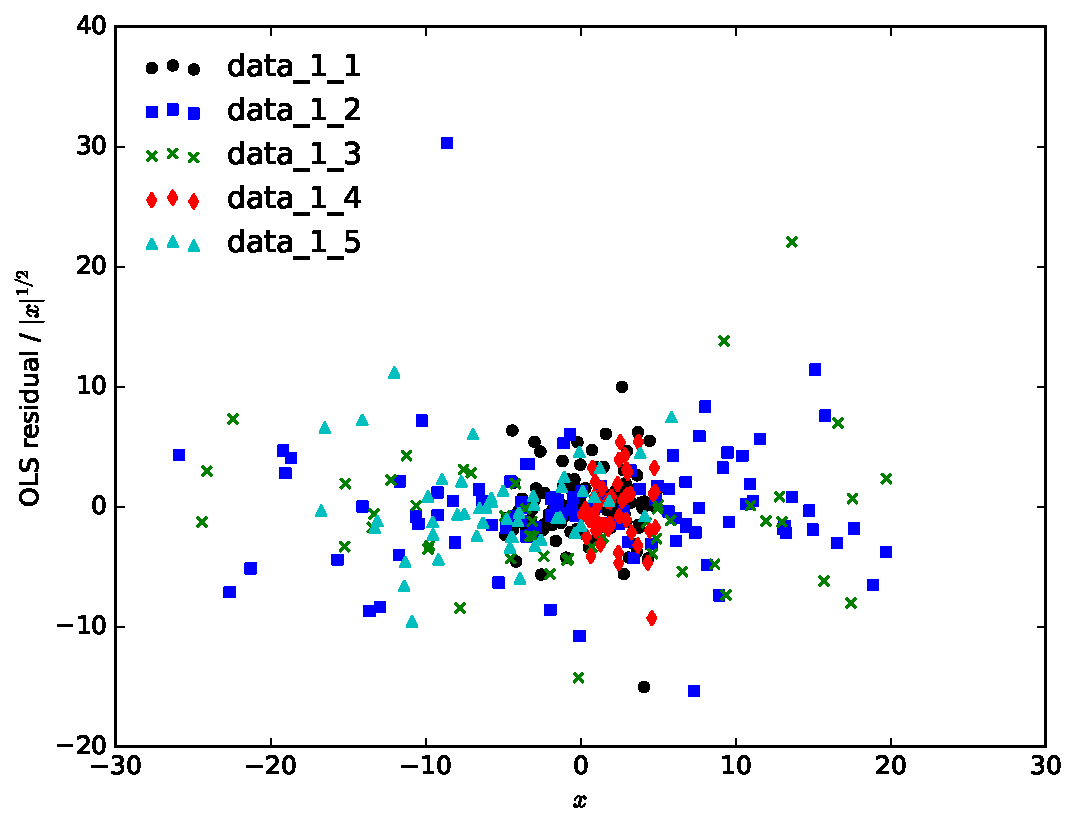
\includegraphics[width=0.7\textwidth]{peek_pattern}
  \caption{$\widehat{e}_i/\left|x_i\right|^{1/2}$as a function of predictors $x_i$'s.}
  \label{fig:pattern}
\end{figure}


\end{document}
